\chapter{Écologie comportementale}\label{ch:b3:behavioural-ecology}

Un suricate se tient debout sur une termitière pendant que le reste de
son groupe creuse pour trouver à manger, et quand un rapace paraît il
aboie et les autres filent vers leurs terriers. La sentinelle a passé
une heure sans manger et s'est faite l'animal le plus visible du désert.
Pourquoi~? Un paon traîne une queue qui lui coûte un cinquième de son
budget énergétique et ralentit sa fuite devant les tigres. Une abeille
qui rentre d'un champ danse sur un rayon vertical, et l'angle de sa
danse à la verticale est l'angle de la nourriture au soleil. Une mésange
charbonnière qui chasse les chenilles dans un bouquet de feuilles le
quitte alors qu'il y reste des chenilles à trouver. Aucun de ces animaux
n'a lu ce chapitre, et pourtant chacun se comporte comme s'il avait
résolu une optimisation, un jeu, ou un problème de comptabilité
familiale. L'écologie comportementale est l'étude du comportement comme
d'un ensemble de solutions évoluées~: à quoi sert un comportement, en
termes de gènes qu'il propage, et quels doivent être ses coûts et ses
bénéfices pour que la sélection naturelle l'ait produit. Ses outils sont
ceux d'un économiste --- l'optimisation, la \omterm{prop:b3:behavioural-ecology:hawk-dove}{théorie des jeux}, la
comptabilité de l'apparentement --- et son épreuve est le terrain.

\section{Quatre questions et la machinerie de l'instinct}

\begin{definition}[Les questions de Tinbergen]\label{def:b3:behavioural-ecology:tinbergen}
\index{les quatre questions de Tinbergen}\index{patron moteur fixe}\index{stimulus déclencheur}\index{empreinte}\index{période critique}
Tinbergen (1963) disait qu'un compte rendu complet d'un comportement
doit répondre à quatre questions~: son \emph{mécanisme} (quels stimulus
et quelle machinerie nerveuse le produisent), son \emph{développement}
(comment il apparaît chez l'individu, à partir des gènes et de
l'expérience), sa \emph{fonction} (comment il contribue à la survie et à
la reproduction) et son \emph{histoire évolutive} (comment il est né
d'un comportement ancestral). Les éthologistes qui les ont formulées
avaient établi les deux premières. Bien des comportements sont des
\emph{patrons moteurs fixes}~: des séquences stéréotypées déclenchées
par un simple \emph{stimulus déclencheur} et menées à leur terme une
fois commencées --- une oie cendrée ramène du bec un œuf déplacé vers le
nid, et achève le mouvement même si l'on retire l'œuf à mi-chemin~; un
poussin de goéland argenté picore une tache rouge sur tout objet en
forme de bec, et picore davantage un bâton à trois bandes rouges que la
tête d'un vrai goéland~; un épinoche mâle attaque tout ce qui est rouge
par-dessous, y compris une camionnette postale qui passe, aperçue par la
fenêtre. D'autres s'apprennent dans une fenêtre~: l'\emph{empreinte},
par laquelle un oison suit dès son premier jour, et traite ensuite comme
son parent, tout ce qui bouge --- une oie, Lorenz, une boîte en carton
--- est rapide, irréversible et confinée à une \emph{période critique}~;
l'apprentissage du chant chez les oiseaux, l'exemple du volume de
deuxième année, a la même forme. La dichotomie de l'inné et de l'acquis
est fausse~: un comportement a un programme génétique qui précise ce
qui doit être appris, quand et de qui, et c'est le programme qui évolue.
\end{definition}

\begin{proof}[Faits expérimentaux]
Les expériences de terrain de Tinbergen ont fixé la méthode. Les guêpes
fouisseuses (\emph{Philanthus}) reviennent à un nid caché dans le
sable~; il déplaça un cercle de pommes de pin qu'il avait posé autour
d'une entrée pendant que la guêpe était partie, et elle chercha au
centre du cercle déplacé --- elle avait appris les repères. Les mouettes
rieuses retirent les coquilles du nid après l'éclosion~; il disposa des
œufs à côté de coquilles peintes, de coquilles naturelles et d'autres
objets, et compta ce que prenaient les corneilles~: la surface interne
blanche d'une coquille attirait les prédateurs, et le retrait qui avait
l'air d'un rangement était un camouflage. Les expériences sur les
poussins de goéland ont quantifié un \omterm{def:b3:behavioural-ecology:tinbergen}{stimulus déclencheur} en offrant des
têtes de carton qui variaient d'un trait à la fois. Les oies imprégnées
de Lorenz le suivirent toute leur vie~; des canetons imprégnés le
premier jour sur une boîte en mouvement ne purent jamais ensuite être
amenés à suivre une cane.
\end{proof}

\begin{omfigure}
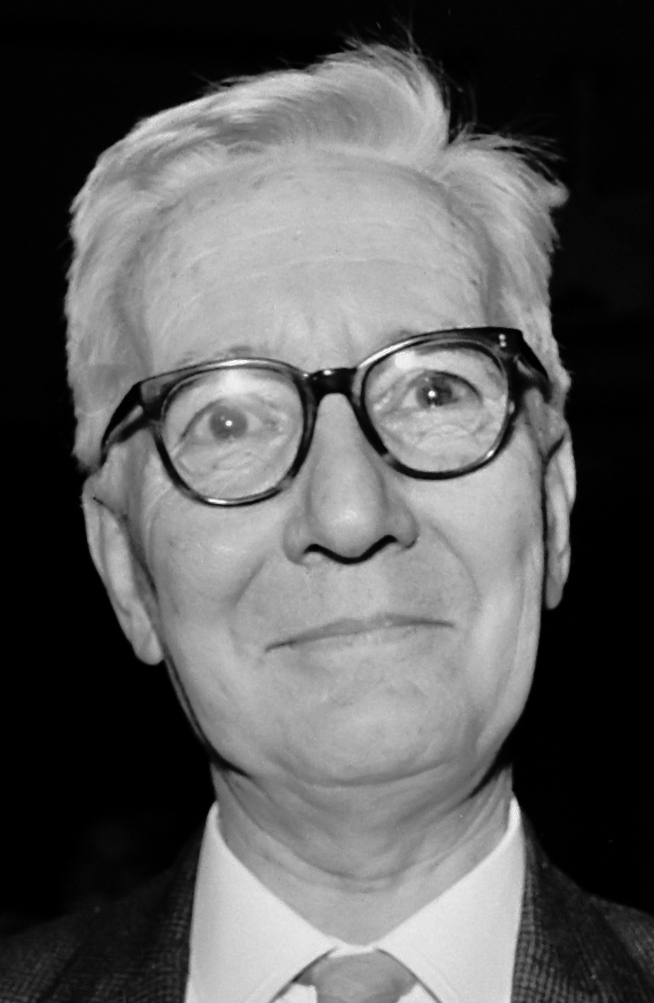
\includegraphics[width=0.36\linewidth]{images/book5/tinbergen.jpg}\hspace{0.04\linewidth}
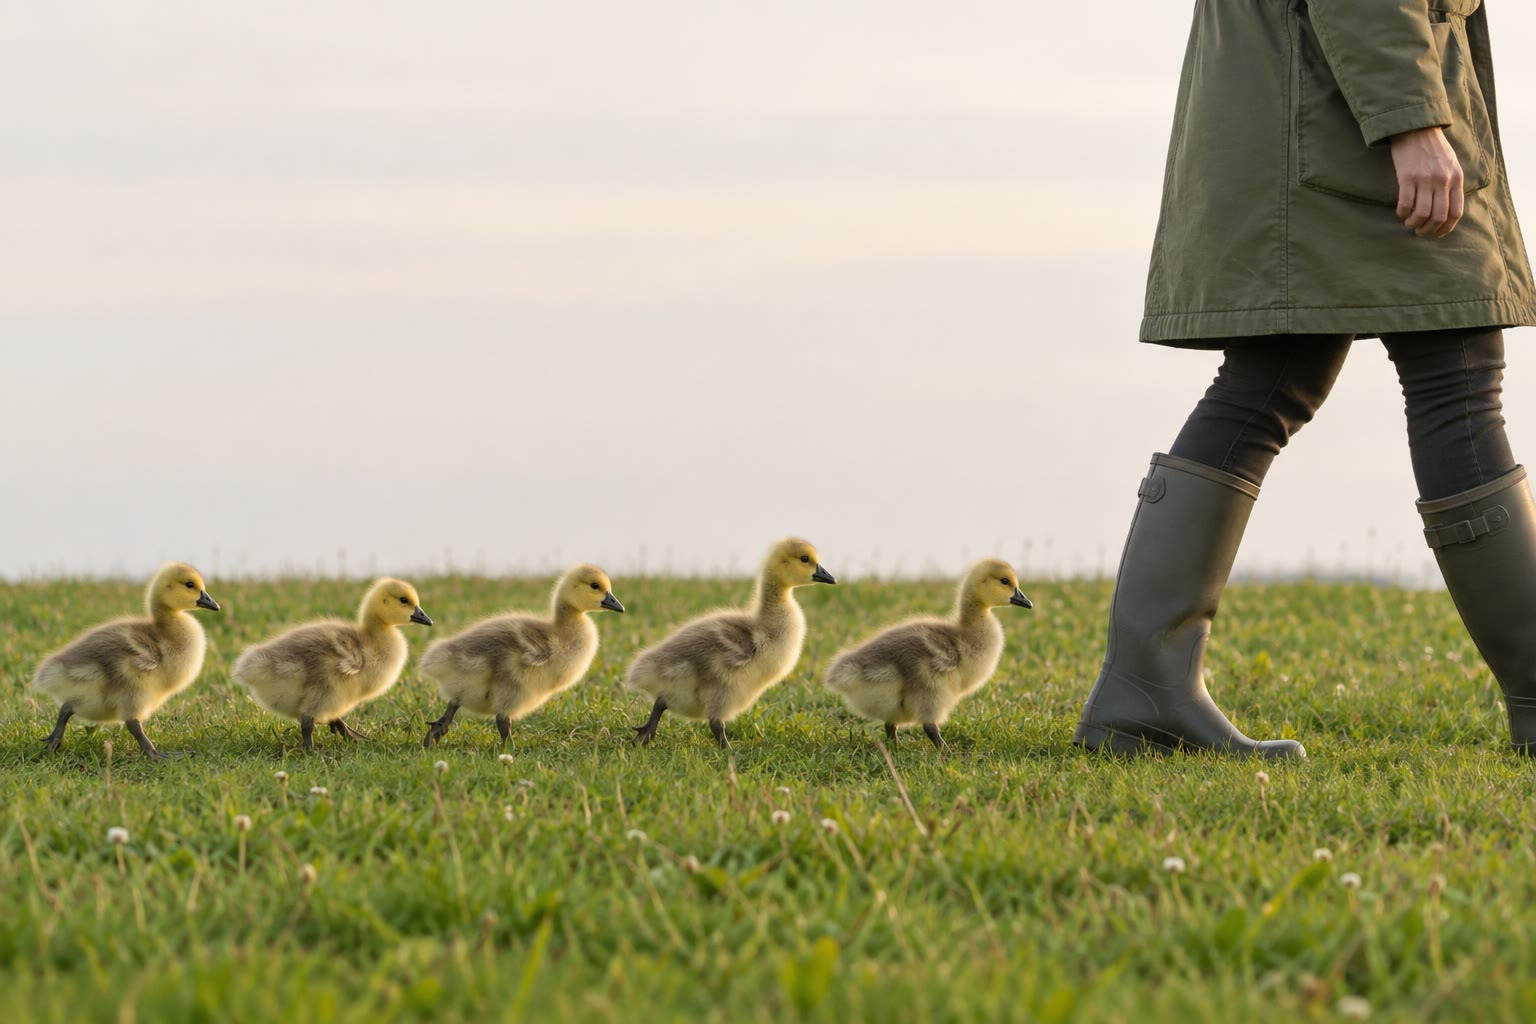
\includegraphics[width=0.52\linewidth]{images/book5/ai/b5-26-goose-imprinting.jpg}

{\small À gauche~: Niko Tinbergen (1907--1988), qui porta les questions
du comportement sur le terrain et les rendit expérimentales
(photographie de Rob Mieremet, Anefo, 1973, CC0). À droite~: des oisons
qui suivent la première grande chose en mouvement qu'ils aient vue, un
jour après l'éclosion, et qu'on ne persuadera jamais du contraire.}
\end{omfigure}

\section{Décider~: la quête optimale}

\begin{theorem}[Le théorème de la valeur marginale]\label{thm:b3:behavioural-ecology:mvt}
\index{quête optimale}\index{théorème de la valeur marginale}\index{temps de séjour dans une parcelle}\index{monnaie}
Un animal en quête visite des parcelles de nourriture séparées par un
temps de trajet $\tau$. Dans une parcelle il gagne une énergie $g(t)$
après un temps $t$, avec $g$ croissante et concave (la parcelle
s'épuise). S'il quitte chaque parcelle après un temps $t$, son taux de
gain à long terme vaut $R(t) = g(t)/(\tau + t)$, et le temps de séjour
$t^{*}$ qui le maximise vérifie
\[
g'(t^{*}) = \frac{g(t^{*})}{\tau + t^{*}} = R(t^{*}) :
\]
quitter une parcelle quand le taux de gain instantané y est tombé au
taux moyen sur tout l'habitat, trajet compris (Charnov, 1976).
Conséquences~: plus le trajet est long, plus le séjour est long et plus
chaque parcelle est épuisée à fond~; dans un habitat plus riche ($R$
plus élevé) chaque parcelle est quittée plus tôt et moins épuisée~; et
toutes les parcelles sont quittées au même taux marginal quelle que soit
leur qualité, de sorte qu'une parcelle pauvre est quittée presque
aussitôt et une riche seulement quand elle a été travaillée jusqu'à la
moyenne de l'habitat. Pour $g(t) = A(1 -
\mathrm{e}^{-t/T_{0}})$ la condition devient $(\tau + t^{*})/T_{0} =
\mathrm{e}^{t^{*}/T_{0}} - 1$, résolue numériquement~: avec $\tau = T_{0}$,
$t^{*} \approx 1.15\,T_{0}$~; avec $\tau = 4T_{0}$, $t^{*} \approx
2.0\,T_{0}$.
\end{theorem}
\begin{proof}
$R(t) = g(t)/(\tau + t)$~; $R'(t) = [g'(t)(\tau + t) - g(t)]/(\tau +
t)^{2} = 0$ donne $g'(t^{*}) = g(t^{*})/(\tau + t^{*})$.
Géométriquement~: tracer $g$ contre $t$ avec l'origine en $-\tau$~;
$R(t)$ est la pente de la droite joignant $(-\tau, 0)$ à $(t, g(t))$,
maximale là où cette droite est tangente à la courbe --- ce qui est la
condition. Un $\tau$ plus grand déplace l'origine vers la gauche et le
point de tangence vers la droite~; un habitat plus riche redresse la
tangente et la déplace vers la gauche. Pour l'exponentielle,
$g' = (A/T_{0})
\mathrm{e}^{-t/T_{0}}$ et $g/(\tau + t) = A(1 - \mathrm{e}^{-t/T_{0}})/
(\tau + t)$~; en égalant et en réarrangeant on obtient l'équation
annoncée, et en y portant $t^{*} = 1.15T_{0}$ avec $\tau = T_{0}$~: à
gauche $2.15$, à droite $\mathrm{e}^{1.15} - 1 = 2.16$.
\end{proof}

\begin{omfigure}
\begin{tikzpicture}
\begin{axis}[
  width=0.68\linewidth, height=5.8cm,
  axis x line=middle, axis y line=left,
  xmin=-4.5, xmax=5, ymin=0, ymax=1.15,
  xlabel={temps (en unités de $T_{0}$)}, ylabel={énergie gagnée dans la parcelle},
  xlabel style={font=\small, at={(axis description cs:0.95,0.0)}, anchor=north}, ylabel style={font=\small},
  tick label style={font=\small}, xtick={-4,-1,0,1.15,2}, xticklabels={$-4T_0$,$-T_0$,0,$1.15$,$2.0$}, ytick={0.5,1}, yticklabels={$0.5A$,$A$},
  clip=false,
]
\addplot[very thick, omDef, domain=0:5, samples=80] {1-exp(-x)};
\draw[thick, omThm] (axis cs:-1,0) -- (axis cs:1.55,1.13);
\draw[thick, omMeth!70!black] (axis cs:-4,0) -- (axis cs:3.5,1.081);
\fill[omThm] (axis cs:1.15,0.6834) circle (2pt); \fill[omMeth!70!black] (axis cs:2,0.8647) circle (2pt);
\draw[dashed, gray] (axis cs:1.15,0) -- (axis cs:1.15,0.6834); \draw[dashed, gray] (axis cs:2,0) -- (axis cs:2,0.8647);
\node[font=\scriptsize, omThm, anchor=north west, align=left] at (axis cs:-4.4,1.1) {trajet court, $\tau = T_{0}$~:\\partir à $t^{*} = 1.15\,T_{0}$,\\parcelle épuisée à \qty{68}{\%}};
\node[font=\scriptsize, omMeth!70!black, anchor=north west, align=left] at (axis cs:2.4,0.62) {trajet long, $\tau = 4T_{0}$~:\\partir à $t^{*} = 2.0\,T_{0}$,\\épuisée à \qty{86}{\%}};
\node[font=\scriptsize, omDef, anchor=north west] at (axis cs:3.0,0.86) {$g(t) = A(1 - \mathrm{e}^{-t/T_{0}})$};
\node[font=\scriptsize, gray, anchor=south] at (axis cs:-2.5,0.02) {trajet};
\end{axis}
\end{tikzpicture}

{\small Le \omterm{thm:b3:behavioural-ecology:mvt}{théorème de la valeur marginale} en image. La courbe de gain
s'aplatit à mesure que la parcelle s'épuise~; la droite joignant le
départ du trajet à un point de la courbe a pour pente le taux de gain
global~; le meilleur moment pour partir est celui où cette droite est
tangente. Un trajet plus long déplace l'origine à gauche et le point de
tangence à droite.}
\end{omfigure}

\begin{proof}[Faits expérimentaux]
Cowie (1977) laissa des mésanges charbonnières chasser des vers de
farine cachés dans des godets remplis de sciure, en volière, le temps de
trajet entre godets étant manipulé par des couvercles plus ou moins
longs à retirer~; les oiseaux restaient plus longtemps dans chaque godet
quand le trajet était plus lent, suivant la prédiction du théorème, et
la dépassaient légèrement dans la direction qu'explique la prise en
compte du coût énergétique du trajet. Des étourneaux qui portaient des
tipules à leurs oisillons (Kacelnik, 1984) prenaient des charges plus
grosses aux mangeoires les plus éloignées, là encore comme l'exige la
solution qui maximise le taux pour une courbe de chargement. Ni l'un ni
l'autre test ne prouve que les oiseaux calculent des tangentes~; tous
deux montrent que la sélection a produit des règles empiriques dont
l'issue est proche de l'optimum.
\end{proof}

\section{Les affrontements~: la théorie des jeux}

\begin{proposition}[Faucon--Colombe et la stratégie évolutivement stable]\label{prop:b3:behavioural-ecology:hawk-dove}
\index{théorie des jeux}\index{jeu Faucon--Colombe}\index{stratégie évolutivement stable}\index{sélection dépendante de la fréquence}
Quand le meilleur comportement dépend de ce que font les autres, il n'y
a pas d'optimum, seulement un \emph{jeu}. Deux animaux se disputent une
ressource de valeur $V$~; un \emph{Faucon} se bat jusqu'à la blessure
(coût $C$) ou la victoire, une \emph{Colombe} parade et se retire si on
l'attaque. Les gains moyens sont
\[
\begin{array}{c|cc}
 & \text{contre Faucon} & \text{contre Colombe}\\ \hline
\text{Faucon} & (V - C)/2 & V\\
\text{Colombe} & 0 & V/2
\end{array}
\]
Une \emph{\omterm{prop:b3:behavioural-ecology:hawk-dove}{stratégie évolutivement stable}} (Maynard Smith et Price, 1973)
est une stratégie qui, une fois répandue, ne peut être envahie par
aucune rare autre. Si $V > C$, Faucon est la SES~: se battre paie même
contre des batailleurs. Si $V
< C$, aucune stratégie pure n'est stable --- une population de Colombes
est envahie par des Faucons, qui gagnent chaque affrontement, et une
population de Faucons par des Colombes, qui évitent les blessures --- et
la SES est de jouer Faucon avec la probabilité
\[
p^{*} = \frac{V}{C},
\]
ou, ce qui revient au même, une population où cette fraction est faite
de Faucons. À la SES les deux stratégies réussissent aussi bien, chacune
gagnant en moyenne $V(1 -
V/C)/2$, moins que le $V/2$ qu'une population de Colombes se serait
partagé~: l'affrontement coûte à tous, et personne ne peut faire mieux
seul. La sélection est ici \emph{dépendante de la fréquence}~: la valeur
sélective d'une stratégie baisse quand elle devient commune, et c'est
pourquoi les affrontements animaux sont surtout des parades et parfois
une guerre, et pourquoi le mélange persiste.
\end{proposition}
\begin{proof}
Soit une fraction $p$ qui joue Faucon. Le gain attendu d'un Faucon vaut
$W_{H} = p(V
- C)/2 + (1 - p)V$~; celui d'une Colombe $W_{D} = (1 - p)V/2$. $W_{H} - W_{D} =
p(V - C)/2 + (1 - p)V/2 = [V - pC]/2$, positif pour $p < V/C$ et négatif
au-dessus~: les Faucons se répandent quand ils sont rares et sont
éliminés quand ils sont communs, et la fréquence se fixe là où
$W_{H} = W_{D}$, en $p^{*} = V/C$. Sa stabilité découle du changement de
signe~: une perturbation de $p$ au-dessus de $p^{*}$ favorise les
Colombes et se corrige, en dessous elle favorise les Faucons. Si $V
\ge C$ la différence est positive pour tout $p \le 1$ et Faucon se fixe.
Le gain commun en $p^{*}$~: $W_{D} = (1 - V/C)V/2$.
\end{proof}

\begin{omfigure}
\begin{tikzpicture}
\begin{axis}[
  width=0.6\linewidth, height=5.4cm,
  axis x line=bottom, axis y line=left,
  xmin=0, xmax=1, ymin=-1, ymax=4.2,
  xlabel={fraction de Faucons $p$}, ylabel={gain attendu},
  xlabel style={font=\small, at={(axis description cs:0.5,-0.12)}, anchor=north}, ylabel style={font=\small},
  tick label style={font=\small}, xtick={0,0.5,1}, xticklabels={0,$p^{*} = V/C$,1}, ytick={0,1,2,4},
  clip=false,
]
\addplot[very thick, omThm, domain=0:1, samples=2] {x*(4-8)/2 + (1-x)*4};
\addplot[very thick, omDef, domain=0:1, samples=2] {(1-x)*4/2};
\draw[dashed, gray] (axis cs:0.5,-1) -- (axis cs:0.5,1);
\fill[black] (axis cs:0.5,1) circle (2pt);
\node[font=\scriptsize, omThm, anchor=north west] at (axis cs:0.5,3.9) {Faucon~: $p(V - C)/2 + (1 - p)V$};
\node[font=\scriptsize, omDef, anchor=south west] at (axis cs:0.62,0.9) {Colombe~: $(1 - p)V/2$};
\node[font=\scriptsize, anchor=west, align=left] at (axis cs:0.55,2.6) {$V = 4$, $C = 8$~:\\SES en $p^{*} = 0.5$,\\gain $V(1 - V/C)/2 = 1$};
\draw[->, thick, omThm] (axis cs:0.1,-0.5) -- (axis cs:0.4,-0.5); \draw[->, thick, omDef] (axis cs:0.9,-0.5) -- (axis cs:0.6,-0.5);
\node[font=\tiny, anchor=north] at (axis cs:0.25,-0.55) {les Faucons se répandent}; \node[font=\tiny, anchor=north] at (axis cs:0.75,-0.55) {les Colombes se répandent};
\end{axis}
\end{tikzpicture}

{\small Le \omterm{prop:b3:behavioural-ecology:hawk-dove}{jeu Faucon--Colombe}. Là où les droites de gain se croisent,
les deux stratégies réussissent aussi bien et aucune ne peut se
répandre~; de part et d'autre, la sélection ramène la fréquence. Le
mélange est stable et coûte à tous, et c'est à cela que ressemblent les
affrontements animaux.}
\end{omfigure}

\begin{example}[Des jeux sur le terrain]\label{ex:b3:behavioural-ecology:games}
Les mâles du tircis se disputent les taches de soleil du sol
forestier~: le résident gagne presque toujours un bref vol en spirale,
et quand on trompe deux mâles pour que chacun se croie résident le
combat dure dix fois plus longtemps --- une convention (« le résident
gagne ») qui règle les affrontements à bon compte, et qui est elle-même
une SES quand se battre coûte cher et que la ressource ne vaut pas
grand-chose. Les mâles de la mouche à bouse attendent les femelles sur
les bouses et repartent quand le rythme des arrivées tombe à ce
qu'offrirait une bouse fraîche --- encore le \omterm{thm:b3:behavioural-ecology:mvt}{théorème de la valeur
marginale}, dans un jeu où la valeur de la parcelle dépend du nombre de
rivaux qui y siègent. Les guêpes des figues, les lézards à taches
latérales dont trois types de mâles se battent cycliquement comme à
pierre--feuille--ciseaux, et les mâles «~resquilleurs~» du saumon et du
crapet arlequin, qui fécondent des œufs en se faufilant devant des mâles
territoriaux qu'ils ne peuvent affronter, sont tous des mélanges tenus à
des fréquences où les solutions de rechange paient également. La guerre
d'usure --- deux animaux qui paradent jusqu'à ce que l'un renonce, la
SES étant de persister pendant un temps tiré d'une loi exponentielle ---
décrit les concours de regard de bien des espèces, et prédit, à juste
titre, que la persistance du perdant ne dit rien de la durée qu'aurait
eue le combat.
\end{example}

\section{La parentèle~: la règle de Hamilton}

\begin{theorem}[La règle de Hamilton]\label{thm:b3:behavioural-ecology:hamilton}
\index{règle de Hamilton}\index{sélection de parentèle}\index{apparentement}\index{valeur sélective inclusive}\index{altruisme}\index{haplodiploïdie}
Un allèle qui pousse son porteur à accomplir un acte lui coûtant $c$
descendants et donnant à un parent $b$ descendants de plus se répand si
\[
r\,b > c ,
\]
où $r$ est le \emph{coefficient d'apparentement}~: la probabilité qu'un
gène du receveur soit une copie, par descendance, du même gène chez
l'acteur --- $1/2$ pour parent et enfant ou pour deux germains, $1/4$
pour des demi-germains, des petits-enfants, des neveux et nièces, $1/8$
pour des cousins germains. La quantité que l'allèle maximise est la
\emph{\omterm{thm:b3:behavioural-ecology:hamilton}{valeur sélective inclusive}} de son porteur~: sa propre
reproduction plus ses effets sur la reproduction de ses apparentés,
chacun pondéré par $r$. L'\emph{altruisme} --- un comportement qui
abaisse la reproduction de l'acteur et élève celle d'un autre ---
évolue donc vers la parentèle, proportionnellement à l'apparentement, et
la règle prédit où on doit le trouver~: dans les cris d'alarme des
femelles de spermophiles, qui vivent parmi leurs sœurs et leurs filles,
et non chez les mâles, qui se dispersent~; dans le tour de garde des
suricates, dont le groupe est une famille~; chez les aides au nid des
oiseaux qui assistent leurs parents à élever des germains quand les
territoires sont pleins. Chez les hyménoptères \emph{haplodiploïdes} ---
mâles issus d'œufs non fécondés avec un seul jeu de chromosomes,
femelles avec deux --- deux sœurs germaines partagent les trois quarts
de leurs gènes ($r = 3/4$), plus qu'une mère n'en partage avec ses
filles ($1/2$), ce que Hamilton proposa comme raison pour laquelle les
castes stériles d'ouvrières des fourmis, des abeilles et des guêpes y
sont apparues onze fois et ailleurs presque jamais.
\end{theorem}
\begin{proof}
Considérons les copies de l'allèle. Quand l'acteur accomplit l'acte, ses
propres copies perdent $c$ en transmission attendue~; le receveur porte
l'allèle avec une probabilité $r$ au-dessus de la moyenne de la
population, de sorte que le gain $b$ du receveur augmente la
transmission de l'allèle de $rb$ en moyenne. L'allèle croît en fréquence
quand $rb - c > 0$ (Hamilton, 1964~; la dérivation générale, à partir de
la covariance entre le génotype d'un individu et sa valeur sélective,
est l'équation de Price, admise ici). L'apparentement~: un parent
transmet chaque gène à un descendant avec la probabilité $1/2$~; deux
germains ont chacun reçu un gène donné du même parent avec la
probabilité $1/2$, et c'est la même copie avec la probabilité $1/2$, et
il y a deux parents~: $r = 2\times\tfrac{1}{2}
\times\tfrac{1}{2} = \tfrac{1}{2}$. Sœurs haplodiploïdes~: de leur père
haploïde elles reçoivent des gènes identiques (probabilité $1$)~; de leur
mère, des copies identiques avec la probabilité $1/2$~; en moyennant sur
les deux parents, $r = (1 + 1/2)/2 = 3/4$.
\end{proof}

\begin{omfigure}
\begin{tikzpicture}[every node/.style={font=\scriptsize}, >=stealth]
  % diploid pedigree
  \node[draw, circle, fill=omDef!30, minimum size=6mm] (m) at (0,3) {}; \node[draw, fill=omDef!30, minimum size=6mm] (f) at (1.6,3) {};
  \node[above, font=\tiny] at (0.8,3.4) {parents diploïdes};
  \draw[thick] (m) -- (f);
  \node[draw, circle, fill=omThm!40, minimum size=6mm] (a) at (0,1.5) {}; \node[draw, circle, fill=omDef!15, minimum size=6mm] (s) at (1.6,1.5) {};
  \draw[thick] (0.8,3) -- (0.8,2.2) -- (0,2.2) -- (a); \draw[thick] (0.8,2.2) -- (1.6,2.2) -- (s);
  \node[draw, circle, fill=omDef!15, minimum size=6mm] (c) at (1.6,0) {}; \draw[thick] (s) -- (c);
  \node[draw, circle, fill=omDef!15, minimum size=6mm] (o) at (0,0) {}; \draw[thick] (a) -- (o);
  \node[left, omThm, font=\tiny] at (-0.4,1.5) {acteur};
  \node[right, font=\tiny] at (1.95,1.5) {germain~: $r = 1/2$};
  \node[right, font=\tiny] at (1.95,0) {nièce~: $r = 1/4$};
  \node[left, font=\tiny] at (-0.4,0) {descendant propre~: $1/2$};
  \node[right, font=\tiny] at (1.95,3) {parent~: $r = 1/2$};
  % haplodiploid
  \begin{scope}[shift={(7.2,0)}]
    \node[draw, circle, fill=omDef!30, minimum size=6mm] (q) at (0,3) {}; \node[draw, fill=omMeth!40, minimum size=6mm] (d) at (1.6,3) {};
    \node[above left, font=\tiny] at (0.1,3.3) {reine (diploïde)}; \node[above right, font=\tiny] at (1.5,3.3) {faux-bourdon (haploïde)};
    \draw[thick] (q) -- (d);
    \node[draw, circle, fill=omThm!40, minimum size=6mm] (w) at (0,1.5) {}; \node[draw, circle, fill=omDef!15, minimum size=6mm] (w2) at (1.6,1.5) {};
    \draw[thick] (0.8,3) -- (0.8,2.2) -- (0,2.2) -- (w); \draw[thick] (0.8,2.2) -- (1.6,2.2) -- (w2);
    \node[left, omThm, font=\tiny] at (-0.4,1.5) {ouvrière};
    \node[right, align=left, font=\tiny] at (1.95,1.5) {sœur germaine~: $r = 3/4$\\(gènes du père identiques,\\ceux de la mère partagés à $1/2$)};
    \node[draw, circle, fill=omDef!15, minimum size=6mm] (wd) at (0,0) {}; \draw[thick] (w) -- (wd);
    \node[right, font=\tiny] at (0.35,0) {fille propre~: $1/2$ --- moins qu'une sœur};
  \end{scope}
  \node[below, align=center] at (4.6,-0.9) {la règle de Hamilton~: aider quand $r\,b > c$~; une ouvrière haplodiploïde qui élève des sœurs\\transmet plus de ses gènes par descendant qu'une qui élève des filles};
\end{tikzpicture}

{\small L'apparentement dans deux sortes de famille. Dans une généalogie
diploïde un germain vaut un demi-descendant~; dans une colonie
haplodiploïde une sœur vaut plus qu'une fille, ce qui fait pencher
l'arithmétique vers rester à la maison pour aider.}
\end{omfigure}

\begin{proof}[Faits expérimentaux]
Sherman (1977) observa des spermophiles de Belding pendant trois étés et
nota qui donnait l'alarme à l'approche des prédateurs~: les femelles
ayant des apparentés à proximité criaient bien plus souvent que celles
qui n'en avaient pas, et que les mâles, qui s'étaient dispersés de leur
lieu de naissance et n'avaient aucun apparenté à portée de voix --- le
crieur attirait l'attention du prédateur, et le payait, seulement quand
il y avait des apparentés à avertir. Les guêpiers à front blanc d'Emlen
aident au nid proportionnellement à l'apparentement, choisissant parmi
les nids disponibles ceux de leurs plus proches parents. L'étude de long
terme des suricates par Clutton-Brock a trouvé que les sentinelles
étaient les individus bien nourris, qui avaient le moins à perdre, et
que la survie du groupe --- et donc celle des apparentés de la
sentinelle --- montait avec l'effort de guet~; le coût, toutefois,
s'est révélé moindre que ne le supposait le récit, puisqu'une sentinelle
sur un monticule est souvent la première au terrier.
\end{proof}

\begin{omfigure}
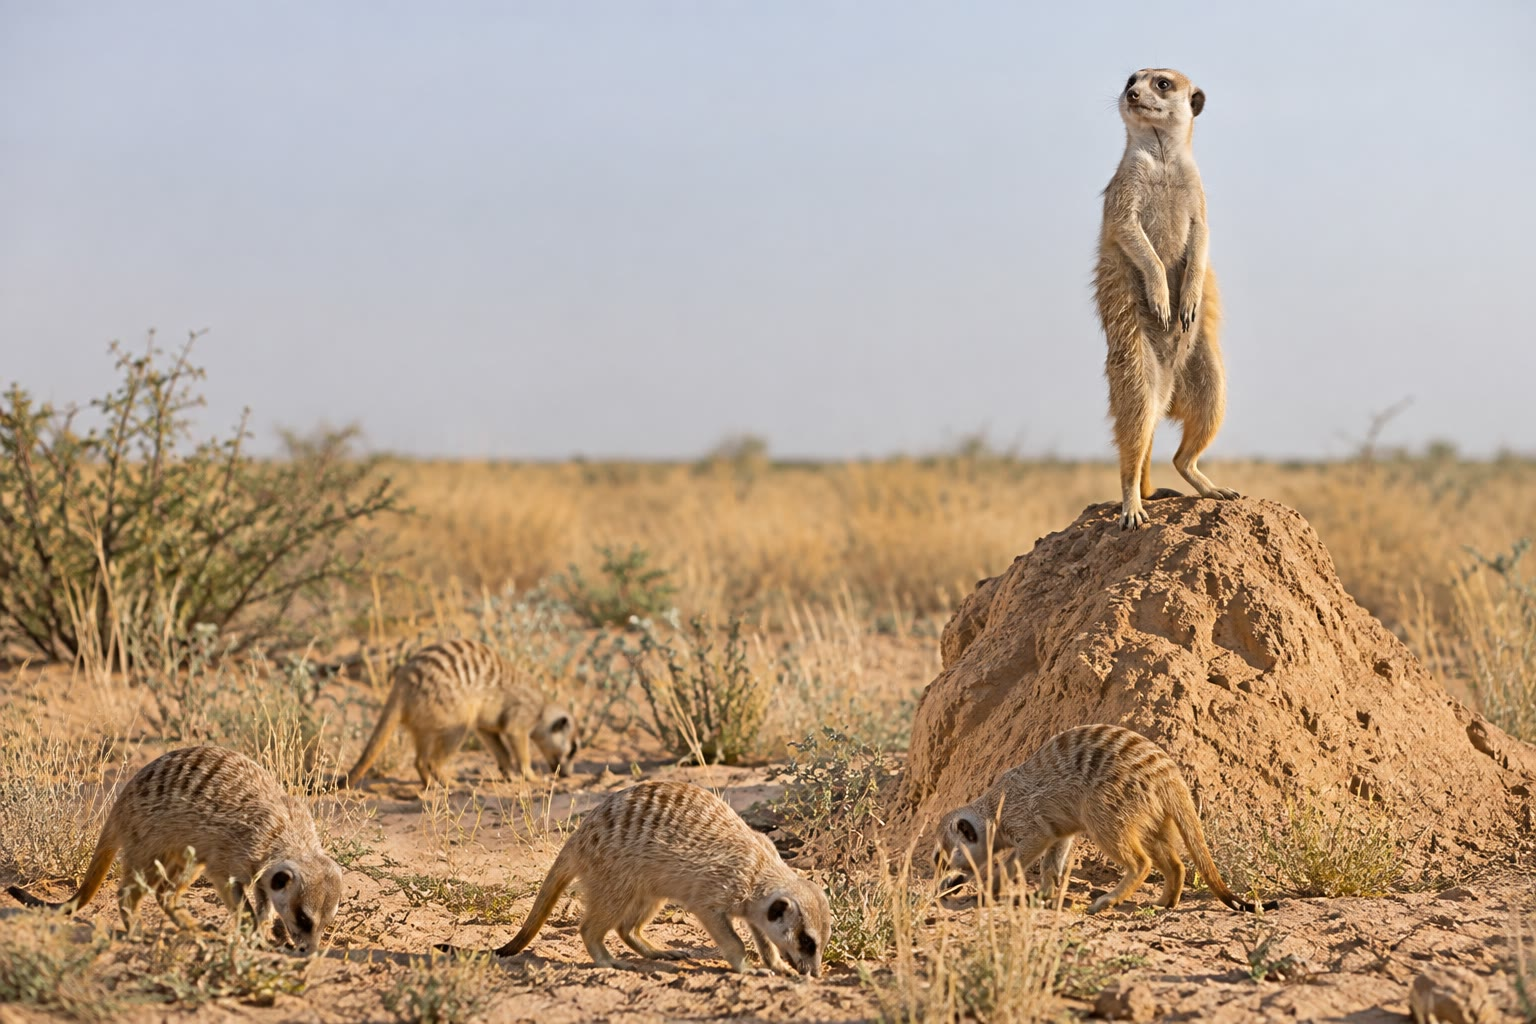
\includegraphics[width=0.46\linewidth]{images/book5/ai/b5-26-meerkat-sentinel.jpg}\hspace{0.04\linewidth}
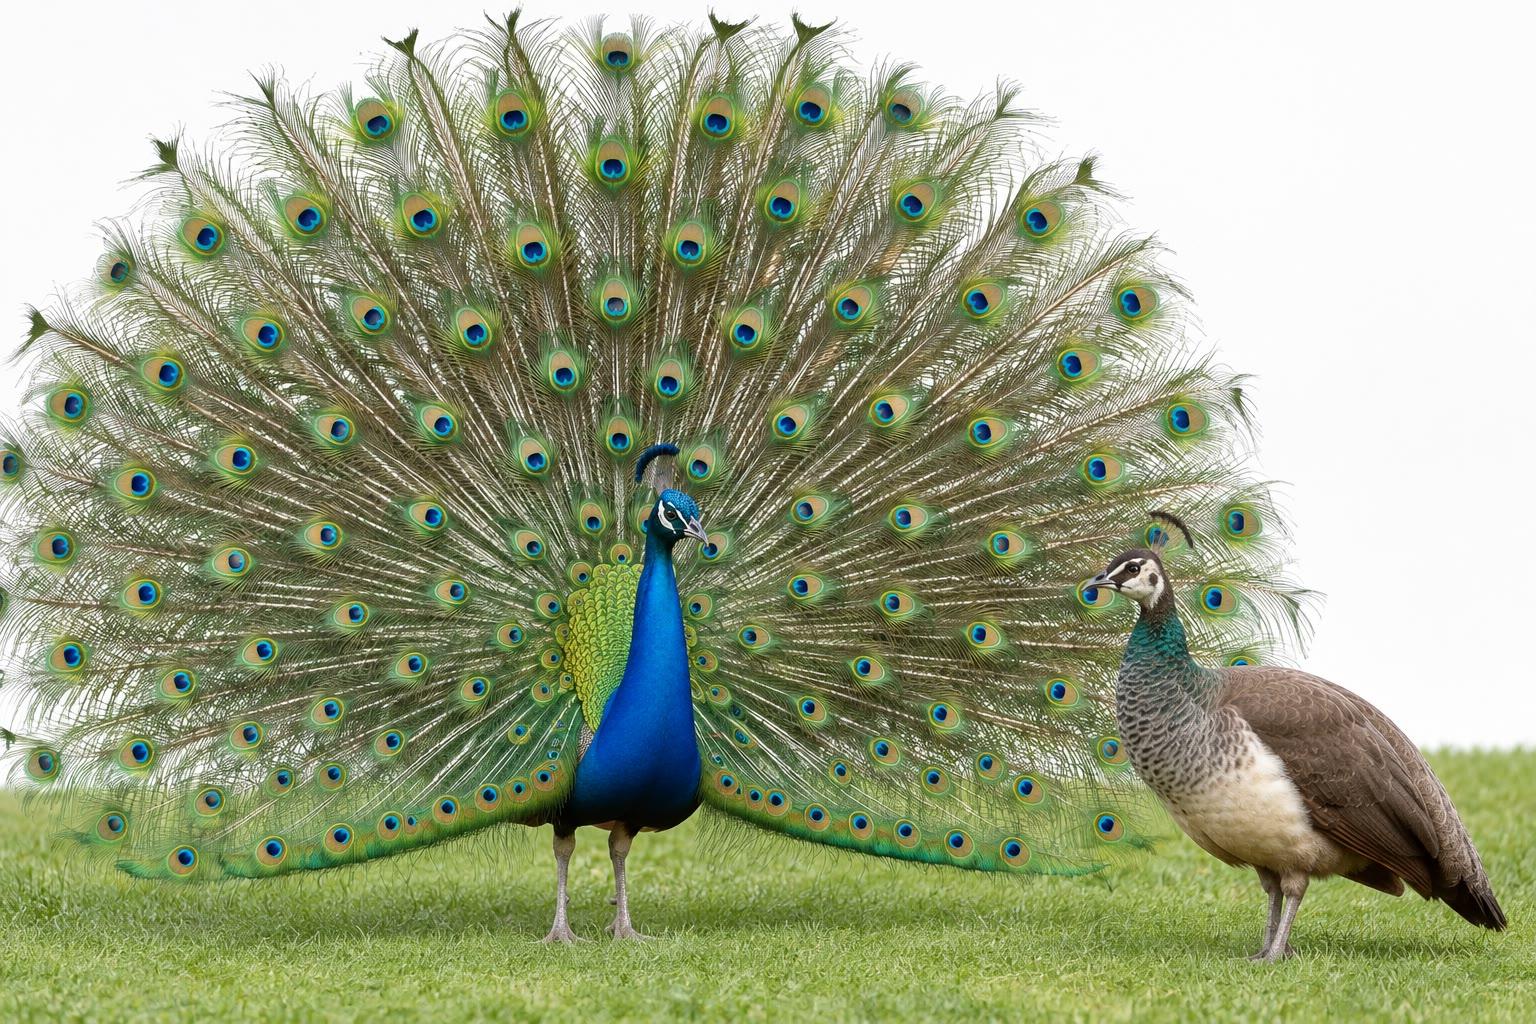
\includegraphics[width=0.46\linewidth]{images/book5/ai/b5-26-peacock-display.jpg}

{\small À gauche~: un suricate en tour de garde au-dessus d'un groupe de
ses apparentés en quête de nourriture. À droite~: un paon qui parade
devant une paonne --- une structure qui coûte à son porteur en nourriture
et en vitesse et ne lui achète rien que l'attention de la femelle.}
\end{omfigure}

\section{Partenaires et messages}

\begin{definition}[La sélection sexuelle]\label{def:b3:behavioural-ecology:sexual-selection}
\index{sélection sexuelle}\index{gradient de Bateman}\index{sélection par emballement}\index{principe du handicap}\index{bons gènes}\index{conflit sexuel}
Le second mécanisme de Darwin~: la sélection sur les traits qui gagnent
des partenaires plutôt que la survie. Sa racine est l'anisogamie --- la
reproduction d'une femelle est limitée par les œufs qu'elle peut
fabriquer et approvisionner, celle d'un mâle par les femelles qu'il peut
féconder --- de sorte que chez la plupart des espèces la valeur
sélective d'un mâle monte fortement avec son nombre d'accouplements et
celle d'une femelle presque pas (le \emph{gradient de Bateman})~; les
mâles rivalisent alors pour les femelles et les femelles choisissent
parmi les mâles. La compétition donne cornes, bois, défenses, grande
taille et les affrontements de la section précédente. Le choix donne les
ornements, et trois explications de la préférence des femelles.
L'\emph{emballement} de Fisher~: une préférence pour une queue un peu
plus longue et la queue plus longue se répandent ensemble, chacune
rendant l'autre avantageuse, jusqu'à ce que le coût de la queue en
survie équilibre son gain en accouplements. Le \emph{handicap} de
Zahavi~: un ornement que seul un mâle en bonne santé peut se permettre
de faire pousser est un \omterm{prop:b3:behavioural-ecology:signals}{signal honnête} de sa condition, précisément
parce qu'il coûte cher --- un paon à la traîne fournie a, de fait, moins
de parasites. Les \emph{bons gènes} et les \emph{bénéfices directs}~: la
femelle y gagne, par l'héritage de sa descendance ou par le territoire
et la nourriture que le mâle fournit. Les intérêts des deux sexes
diffèrent, et le \emph{conflit sexuel} --- sur la fréquence des
accouplements, sur qui soigne les jeunes, sur le sort du sperme d'un
partenaire précédent --- est une course aux armements menée au sein
d'une espèce~: le liquide séminal des mouches du vinaigre mâles
raccourcit la vie de la femelle et élève sa ponte, et les femelles
acquièrent une résistance.
\end{definition}

\begin{proof}[Faits expérimentaux]
Andersson (1982) coupa et recolla les plumes de la queue de veuves à
longue queue mâles au Kenya~: les mâles à queue rallongée au double de
sa longueur naturelle attiraient sur leurs territoires quatre fois plus
de nids nouveaux que les mâles à queue raccourcie, tandis que les
témoins, dont la queue avait été coupée et recollée sans changement,
n'étaient pas affectés --- la préférence des femelles va à une queue
plus longue que celle d'aucun mâle, la signature d'une préférence
sélectionnée au-delà du trait. Petrie (1994) trouva que les paonnes
s'accouplaient aux mâles dont la traîne portait le plus d'ocelles, et
que les poussins de ces mâles survivaient mieux dans les bois où on les
relâchait --- un bénéfice de \omterm{def:b3:behavioural-ecology:sexual-selection}{bons gènes} mesuré. Bateman (1948) compta
les accouplements et les descendants de mouches du vinaigre porteuses
de mutations marqueuses et trouva le gradient qui porte son nom~: le
succès reproducteur des mâles montait linéairement avec les
accouplements, celui des femelles plafonnait après un seul.
\end{proof}

\begin{proposition}[Les signaux honnêtes]\label{prop:b3:behavioural-ecology:signals}
\index{communication}\index{signal honnête}\index{danse frétillante}\index{signal référentiel}
Un signal est un acte qui change le comportement d'un receveur et qui a
évolué pour cela~; il n'est stable que s'il paie aux deux parties, en
moyenne, d'émettre et de répondre. Là où les deux ont des intérêts
communs le signal peut être bon marché et précis~: la \emph{\omterm{prop:b3:behavioural-ecology:signals}{danse
frétillante}} d'une abeille butineuse (von Frisch, dans les années 1940)
code la direction d'une source de nourriture par l'angle de la course
frétillante à la verticale --- l'angle de la source au soleil --- et sa
distance par la durée de la course, environ une seconde par kilomètre,
et les recrues volent à quelques dizaines de mètres de la cible~; les
singes vervets donnent des cris d'alarme distincts pour les léopards,
les aigles et les serpents, et les auditeurs réagissent comme il
convient à chaque cri diffusé par un haut-parleur caché --- des signaux
\emph{référentiels}. Là où les intérêts s'opposent, un signal doit être
coûteux ou infalsifiable pour rester honnête --- le brame d'un cerf,
dont seul un cerf en forme peut soutenir le rythme~; la taille du coassement
d'un crapaud, fixée par son corps~; les ornements du paragraphe
précédent --- sinon il est exploité~: des lucioles d'un genre imitent
les éclairs des femelles d'un autre pour manger les mâles qui viennent,
et la quémande des poussins de coucou surenchérit sur celle des jeunes
de l'hôte. La théorie du signal prédit ainsi la forme d'un signal
d'après la relation entre les parties~: bon marché et informatif entre
apparentés et partenaires dont les intérêts coïncident, coûteux et
ritualisé entre rivaux, et une course aux armements entre prédateur et
proie.
\end{proposition}
\admitted

\begin{omfigure}
\begin{tikzpicture}[every node/.style={font=\scriptsize}, >=stealth]
  % field view
  \node[above] at (0,3.2) {sur le terrain};
  \draw[->, thick, gray] (0,0) -- (0,2.6) node[above, font=\tiny] {vers le soleil};
  \fill[omDef!60] (0,0) circle (0.12); \node[below, font=\tiny] at (0,-0.2) {ruche};
  \draw[->, very thick, omThm] (0,0) -- ({2.4*sin(40)},{2.4*cos(40)}); \node[right, font=\tiny, omThm] at ({2.4*sin(40)},{2.4*cos(40)}) {nourriture, \qty{1}{km}};
  \draw[omThm] (0,1.0) arc[start angle=90, end angle=50, radius=1.0]; \node[font=\tiny, omThm] at (0.55,1.25) {$40^{\circ}$};
  % comb view
  \begin{scope}[shift={(6.2,0)}]
    \node[above] at (0,3.2) {sur le rayon vertical};
    \draw[very thick, gray!60] (-1.8,-0.4) rectangle (1.8,3.0);
    \draw[->, thick, gray] (0,0) -- (0,2.6) node[above, font=\tiny] {le haut (= le soleil)};
    \draw[->, very thick, omThm] (0,0) -- ({1.6*sin(40)},{1.6*cos(40)}); \node[below, align=center, font=\tiny, omThm] at (0,-0.5) {course frétillante~: $40^{\circ}$ par rapport à la verticale~;\\durée $\approx \qty{1}{s}$ par km};
    \draw[omThm, dashed] ({1.6*sin(40)},{1.6*cos(40)}) .. controls (1.3,0.4) and (0.5,-0.3) .. (0,0);
    \draw[omThm, dashed] ({1.6*sin(40)},{1.6*cos(40)}) .. controls (-0.2,1.2) and (-0.6,0.3) .. (0,0);
    \draw[omThm] (0,0.8) arc[start angle=90, end angle=50, radius=0.8]; \node[font=\tiny, omThm] at (0.45,1.0) {$40^{\circ}$};
  \end{scope}
  \node[right, align=left] at (9.2,1.3) {un code symbolique~: la pesanteur\\tient lieu du soleil, le temps\\de la distance~; les recrues arrivent\\à quelques dizaines de mètres près};
\end{tikzpicture}

{\small La \omterm{prop:b3:behavioural-ecology:signals}{danse frétillante}. L'angle de la course à la verticale est
l'angle de la nourriture au soleil~; la longueur de la course est la
distance. Un signal aussi bon marché et aussi précis est possible parce
que la danseuse et son public sont des sœurs de même intérêt.}
\end{omfigure}

\begin{omfigure}
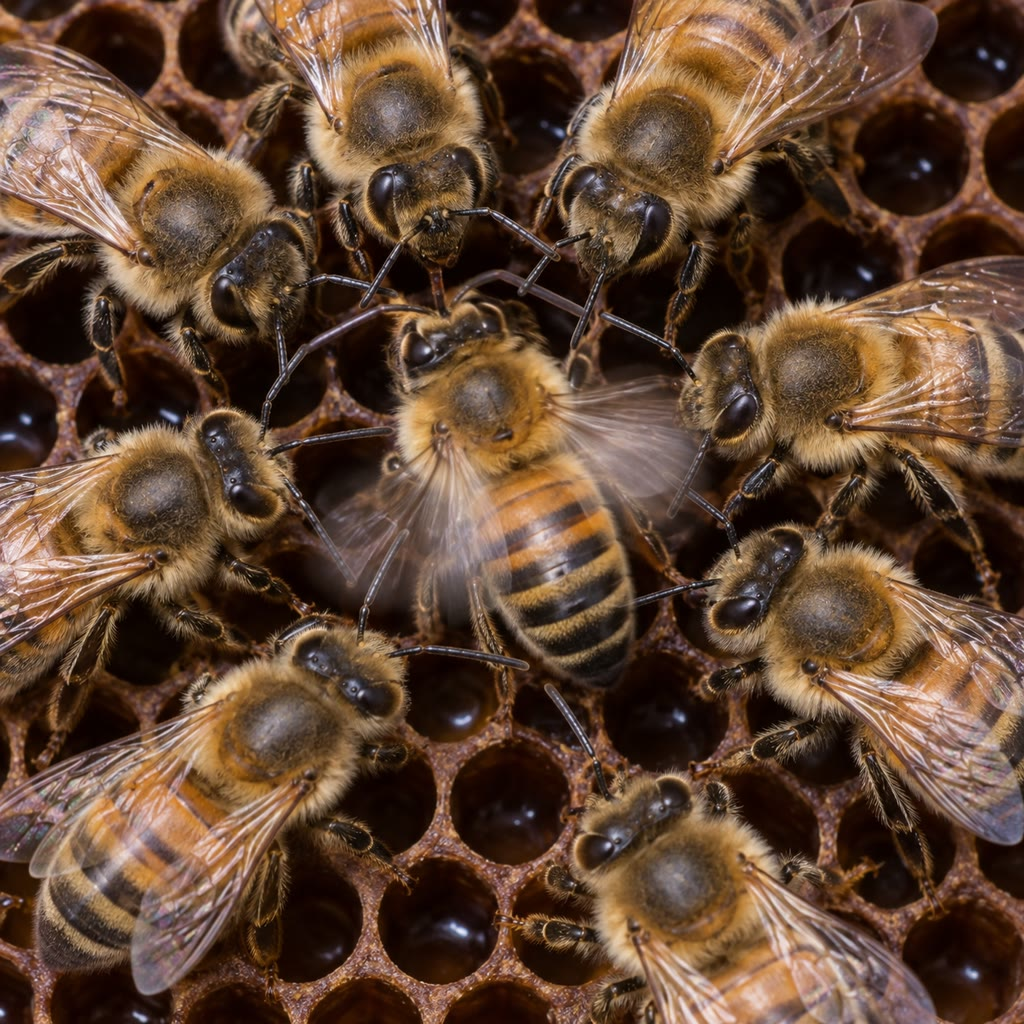
\includegraphics[width=0.4\linewidth]{images/book5/ai/b5-26-bee-dance.jpg}

{\small Une butineuse qui danse sur le rayon, entourée d'ouvrières qui
lisent l'angle et le tempo de sa course.}
\end{omfigure}

\begin{remark}[Pourquoi les animaux semblent calculer]\label{rem:b3:behavioural-ecology:remark}
La mésange charbonnière ne dérive pas $g(t)/(\tau + t)$, le suricate ne
calcule pas $r$, et la paonne n'a jamais entendu parler de handicap.
Chacun porte des règles --- partir quand les captures ralentissent,
crier quand le groupe est la famille, préférer le plus brillant --- que
la sélection a façonnées parce que les animaux qui les suivaient
laissaient plus de descendants~; la mathématique est la nôtre, une façon
de demander ce que les règles doivent accomplir pour qu'il en soit
ainsi, et de prédire le comportement dans des situations que les animaux
n'ont jamais rencontrées. Quand les prédictions échouent --- la mésange
reste trop longtemps, le coût de la sentinelle est moindre qu'on ne le
supposait --- l'échec est instructif~: une monnaie était fausse, une
contrainte avait été oubliée, un apparenté mal compté. La discipline est
une conversation, décennie après décennie, entre un carnet de terrain et
une ligne d'algèbre, et les quatre questions que Tinbergen a posées
restent le cadre des deux.
\end{remark}

\section{Exercices}

\begin{exercise}[$\star$]\label{exo:b3:behavioural-ecology:1}
Énoncer \omterm{def:b3:behavioural-ecology:tinbergen}{les quatre questions de Tinbergen} et répondre à chacune, en une
phrase, pour la \omterm{prop:b3:behavioural-ecology:signals}{danse frétillante}.
\end{exercise}

\begin{exercise}[$\star$]\label{exo:b3:behavioural-ecology:2}
Qu'est-ce qu'un \omterm{def:b3:behavioural-ecology:tinbergen}{patron moteur fixe} et un \omterm{def:b3:behavioural-ecology:tinbergen}{stimulus déclencheur}~? En
donner deux exemples et expliquer ce qu'a montré le bâton
«~supranormal~» à trois bandes rouges.
\end{exercise}

\begin{exercise}[$\star$]\label{exo:b3:behavioural-ecology:3}
Avec des mots, que dit le \omterm{thm:b3:behavioural-ecology:mvt}{théorème de la valeur marginale}, et que
prédit-il de l'usage des parcelles quand le temps de trajet double~?
\end{exercise}

\begin{exercise}[$\star$]\label{exo:b3:behavioural-ecology:4}
Définir une SES. Pourquoi une population de Colombes pures n'en est-elle
pas une, et pourquoi le mélange Faucon--Colombe coûte-t-il à tous~?
\end{exercise}

\begin{exercise}[$\star\star$]\label{exo:b3:behavioural-ecology:5}
Faucon--Colombe avec $V = 6$, $C = 10$~: calculer $p^{*}$, le gain de
chaque stratégie à la SES, et le gain qu'aurait une population de
Colombes pures. Refaire pour $V = 12$, $C = 10$.
\end{exercise}

\begin{exercise}[$\star\star$]\label{exo:b3:behavioural-ecology:6}
Une fonction de gain $g(t) = A(1 - \mathrm{e}^{-t/T_{0}})$ avec $T_{0} =
\qty{2}{min}$. Trouver $t^{*}$ pour $\tau = 2$ et $\tau = 8$ minutes
(employer les valeurs du chapitre), la fraction consommée de chaque
parcelle, et le taux à long terme $R$ en fraction d'$A$ par minute.
\end{exercise}

\begin{exercise}[$\star\star$]\label{exo:b3:behavioural-ecology:7}
Calculer $r$ entre~: des demi-germains~; grand-parent et petit-enfant~;
des cousins germains~; une ouvrière haplodiploïde et son frère~; une
reine haplodiploïde et son fils. Expliquer les deux derniers.
\end{exercise}

\begin{exercise}[$\star\star$]\label{exo:b3:behavioural-ecology:8}
Un cri d'alarme coûte au crieur \qty{2}{\%} de risque de mort et épargne
à chacun de $n$ apparentés voisins un risque de \qty{1}{\%}. Pour quels
$n$ la \omterm{thm:b3:behavioural-ecology:hamilton}{règle de Hamilton} favorise-t-elle le cri si les apparentés sont
des germains~? Des nièces~? Des non-apparentés~?
\end{exercise}

\begin{exercise}[$\star\star$]\label{exo:b3:behavioural-ecology:9}
La queue d'une veuve à longue queue fait \qty{50}{cm}~; rallongée à
\qty{75}{cm} elle attire deux fois plus de nids, raccourcie à
\qty{25}{cm} deux fois moins. Si la survie baisse de \qty{20}{\%} par
tranche de \qty{25}{cm} ajoutée, quelle queue maximise le produit des
accouplements et de la survie, et pourquoi la queue naturelle
pourrait-elle être plus courte~?
\end{exercise}

\begin{exercise}[$\star\star\star$]\label{exo:b3:behavioural-ecology:10}
Ajouter une troisième stratégie, Riposteur, qui parade comme une
Colombe mais riposte si on l'attaque. Écrire ses gains contre Faucon,
Colombe et lui-même (contre Faucon il se bat~: $(V - C)/2$~; contre
Colombe et Riposteur il partage~: $V/2$). Montrer qu'une population de
Riposteurs ne peut être envahie par des Faucons quand $V < C$, et
discuter si des Colombes peuvent y dériver.
\end{exercise}

\begin{exercise}[$\star\star\star$]\label{exo:b3:behavioural-ecology:11}
Dans une guerre d'usure, chaque adversaire persiste pendant un temps
tiré d'une loi~; la SES est exponentielle de moyenne $V/$(coût par unité
de temps). Expliquer pourquoi un temps de persistance fixe ne peut être
une SES, et pourquoi une loi exponentielle rend la persistance future
attendue d'un adversaire encore en parade indépendante du temps qu'il a
déjà paradé.
\end{exercise}

\begin{exercise}[$\star\star\star$]\label{exo:b3:behavioural-ecology:12}
L'argument de Hamilton sur l'haplodiploïdie prédit que les ouvrières
devraient préférer élever des sœurs ($r = 3/4$) plutôt que des frères
($r = 1/4$), tandis que la reine accorde la même valeur à ses fils et à
ses filles. Prévoir le sex-ratio des reproducteurs qu'une colonie
devrait produire si les ouvrières le contrôlent, et si la reine le
contrôle~; dire ce qu'ont trouvé Trivers et Hare, et ce qu'une reine
accouplée à plusieurs mâles fait à l'argument.
\end{exercise}

\section{Problème~: l'arithmétique de la sentinelle}

\begin{problem}[{Problème du week-end --- une journée dans un groupe de
suricates traitée en écologie comportementale~: les temps de parcelle du
théorème de la valeur marginale, les affrontements du jeu
Faucon--Colombe et sa SES, la comptabilité de parentèle du tour de garde
et d'une ruche haplodiploïde, et le coût d'un ornement, pour finir sur
le temps de séjour, la fréquence des Faucons et le seuil de Hamilton de
la sentinelle}]
\label{pb:b3:behavioural-ecology:1}
Données~: des parcelles de quête avec $g(t) = A(1 - \mathrm{e}^{-t/T_{0}})$, $T_{0}
= \qty{3}{min}$, $A = \qty{60}{kJ}$~; trajet entre parcelles $\tau =
\qty{3}{min}$ (habitat dense) ou \qty{12}{min} (clairsemé).
Affrontements pour un terrier~: $V = 10$, $C = 30$ (en unités de valeur
sélective). Sentinelle~: une heure de garde coûte à la sentinelle
$c = 0.03$ équivalent-descendant (nourriture perdue, exposition)~; elle
abaisse le risque de prédation de chaque membre du groupe, ce qui vaut
$b = 0.01$ équivalent-descendant chacun~; le groupe a $n$ membres
d'apparentement moyen $\bar r$. Ruche~: une ouvrière peut élever soit $k$
sœurs, soit $k$ filles à elle pour le même effort. Ornement~: une
longueur de queue $L$ donne des accouplements $m(L) = L/20$ et une
survie $s(L) = 1 - (L/100)^{2}$, $L$ en cm.

\medskip
\noindent\textbf{Partie I --- Les parcelles.}
\begin{enumerate}
  \item Écrire le taux à long terme $R(t)$ et la condition de valeur
        marginale pour ce $g$.
  \item Montrer que la condition se réduit à $(\tau + t)/T_{0} = \mathrm{e}^{t/T_{0}}
        - 1$, et la résoudre pour $\tau = T_{0}$ (essayer $t = 1.15\,T_{0}$).
  \item La résoudre pour $\tau = 4T_{0}$ (essayer $t = 2.0\,T_{0}$).
  \item Pour chaque cas~: temps de séjour en minutes, énergie par
        parcelle, fraction consommée de la parcelle, et taux $R$ en
        kJ/min.
  \item Une règle empirique~: «~partir après \qty{5}{min} fixes~».
        Calculer $R$ pour les deux habitats et comparer à l'optimum. La
        règle est-elle assez bonne~?
  \item Une autre règle~: «~partir quand \qty{20}{s} passent sans
        capture~». Expliquer pourquoi cette règle du temps d'abandon
        approche le théorème, et dans quel sens elle échoue quand les
        parcelles diffèrent en richesse.
\end{enumerate}

\medskip
\noindent\textbf{Partie II --- Les affrontements.}
\begin{enumerate}[resume]
  \item Écrire la matrice des gains et calculer $p^{*}$.
  \item Gain du Faucon et de la Colombe quand $p = 0.1$, $p = p^{*}$ et $p =
        0.6$~; quelle stratégie se répand dans chaque cas~?
  \item Gain à la SES~; comparer au gain de la population de Colombes
        pures. Combien la population perd-elle par affrontement à cause
        de la possibilité de se battre~?
  \item Une sécheresse porte $V$ à $40$ (terriers rares). Nouvelle SES~?
        Que cela prédit-il des combats dans les années difficiles~?
  \item Bourgeois~: «~Faucon si résident, Colombe si intrus~», chaque
        rôle la moitié du temps. Son gain contre lui-même vaut $V/2$ sans
        combat. Montrer que les Faucons ne peuvent envahir une population
        de Bourgeois quand $V
        < C$, et expliquer le cas du tircis.
  \item Expliquer en une phrase pourquoi c'est la dépendance à la
        fréquence, et non un optimum, qui gouverne ce comportement.
\end{enumerate}

\medskip
\noindent\textbf{Partie III --- La parentèle.}
\begin{enumerate}[resume]
  \item La \omterm{thm:b3:behavioural-ecology:hamilton}{règle de Hamilton} pour la sentinelle~: condition sur $n\bar r$.
        Pour quel $n\bar r$ la garde paie-t-elle~?
  \item Un groupe de $n = 8$ germains ($\bar r = 1/2$)~: cela paie-t-il~?
        Un groupe de 8 animaux non apparentés~? Un groupe de 8
        demi-germains~?
  \item La sentinelle est bien nourrie, si bien que son $c$ tombe à
        $0.01$. Quel seuil maintenant~? Pourquoi cela prédit-il que les
        sentinelles sont les individus bien nourris~?
  \item La ruche~: valeur en \omterm{thm:b3:behavioural-ecology:hamilton}{valeur sélective inclusive} de $k$ sœurs
        contre $k$ filles. Que devrait préférer une ouvrière, et dans
        quel rapport~?
  \item La reine s'est accouplée avec trois mâles à parts égales~:
        apparentement moyen des ouvrières à leurs sœurs~? La préférence
        survit-elle~?
  \item Expliquer pourquoi la \omterm{thm:b3:behavioural-ecology:hamilton}{règle de Hamilton} n'exige pas que l'acteur
        reconnaisse ses apparentés, et quelle règle empirique un
        spermophile pourrait employer en pratique.
\end{enumerate}

\medskip
\noindent\textbf{Partie IV --- Les ornements.}
\begin{enumerate}[resume]
  \item Valeur sélective $W(L) = m(L)\,s(L)$. Calculer $W$ pour $L = 20$,
        $40$, $60$, $80$.
  \item Trouver analytiquement le $L$ qui maximise $W$, et $W$ en ce
        point.
  \item Le coût en survie se durcit en $s = 1 - (L/70)^{2}$ (un prédateur
        arrive). Nouvel optimum~? Dans quel sens, et pourquoi cela
        prédit-il que l'évolution de la queue suit la prédation~?
  \item L'expérience d'Andersson a doublé les queues à \qty{75}{cm} et
        doublé les nids. La préférence des femelles pour des queues plus
        longues, «~au-delà de l'optimum~», est-elle compatible avec
        l'explication par l'emballement, avec celle par le handicap, ou
        avec les deux~?
  \item Pourquoi un ornement bon marché n'est-il pas un \omterm{prop:b3:behavioural-ecology:signals}{signal honnête},
        et comment le coût de la question~21 en fait-il un~?
  \item \omterm{def:b3:behavioural-ecology:sexual-selection}{Gradients de Bateman}~: les mâles gagnent $0.8$ descendant par
        accouplement supplémentaire, les femelles $0.1$. Expliquer en un
        paragraphe comment cette asymétrie engendre à la fois les
        affrontements de la partie~II et les ornements de la partie~IV.
  \item Résumer~: $t^{*}$ dans l'habitat dense (question~4), $p^{*}$
        (question~7), et le seuil $n\bar r$ de la sentinelle
        (question~13).
\end{enumerate}
\end{problem}
